\documentclass[aps,prd,onecolumn,nofootinbib,superscriptaddress]{revtex4-2}

\usepackage{amsmath,amssymb,graphicx,xcolor,listings,hyperref,float}

\hypersetup{
    colorlinks=true,
    linkcolor=blue,
    citecolor=blue,
    urlcolor=blue
}

\begin{document}

\title{A Universal Entropy Bridge Between QCD and Gravity:\\
Linking the 9.81\,k$_B$ Constant to Black Hole Thermodynamics}

\author{Johann Anton Michael Tupay}
\affiliation{London, United Kingdom}

\date{\today}

\begin{abstract}
We show that the universal QCD renormalization-group entropy drop
$\Delta S_{\mathrm{RG}} \approx 9.81\,k_B$, derived in Paper~5 from continuum
field theory, is directly related to the Bekenstein--Hawking entropy of
a black hole of the same mass as a neutron star at the QCD entropy ceiling.
The ratio $S_{\mathrm{BH}} / S_{\mathrm{QCD}}$ is given in closed form entirely
in terms of fundamental constants (proton mass, Planck mass, $\Delta S_{\mathrm{RG}}$),
with no astrophysical inputs. This provides a direct link between the
strong-interaction entropy bound and gravitational information bounds,
uniting microphysics and macrophysics in a testable way.
\end{abstract}

\maketitle

\section{Introduction}

Papers~1--5 in this series established the $\Delta S_{\mathrm{RG}} \approx 9.81\,k_B$ constant as:
(i) the origin of hadron masses~\cite{paper1,weinberg1972,collins1974},
(ii) a filter for allowed exotic hadrons~\cite{paper2,esposito2017,brambilla2020},
(iii) the threshold for quark--gluon plasma formation~\cite{paper3,bazavov2014,borsanyi2014},
(iv) a density cutoff in neutron star equations of state~\cite{paper4,ozel2016,lattimer2007},
and (v) a quantity derivable from continuum QFT anomalies~\cite{paper5,casini2011,komargodski2011}.

Here we extend the universality of $\Delta S_{\mathrm{RG}}$ by showing that it
sets the proportionality between the entropy of an object at the QCD ceiling
and the Bekenstein--Hawking entropy of a black hole of the same mass.
This relation involves only fundamental constants, offering a bridge between
QCD thermodynamics and gravitational thermodynamics~\cite{bekenstein1973,hawking1975,misner1973,wald1984}.

\begin{figure}[htbp]
\centering
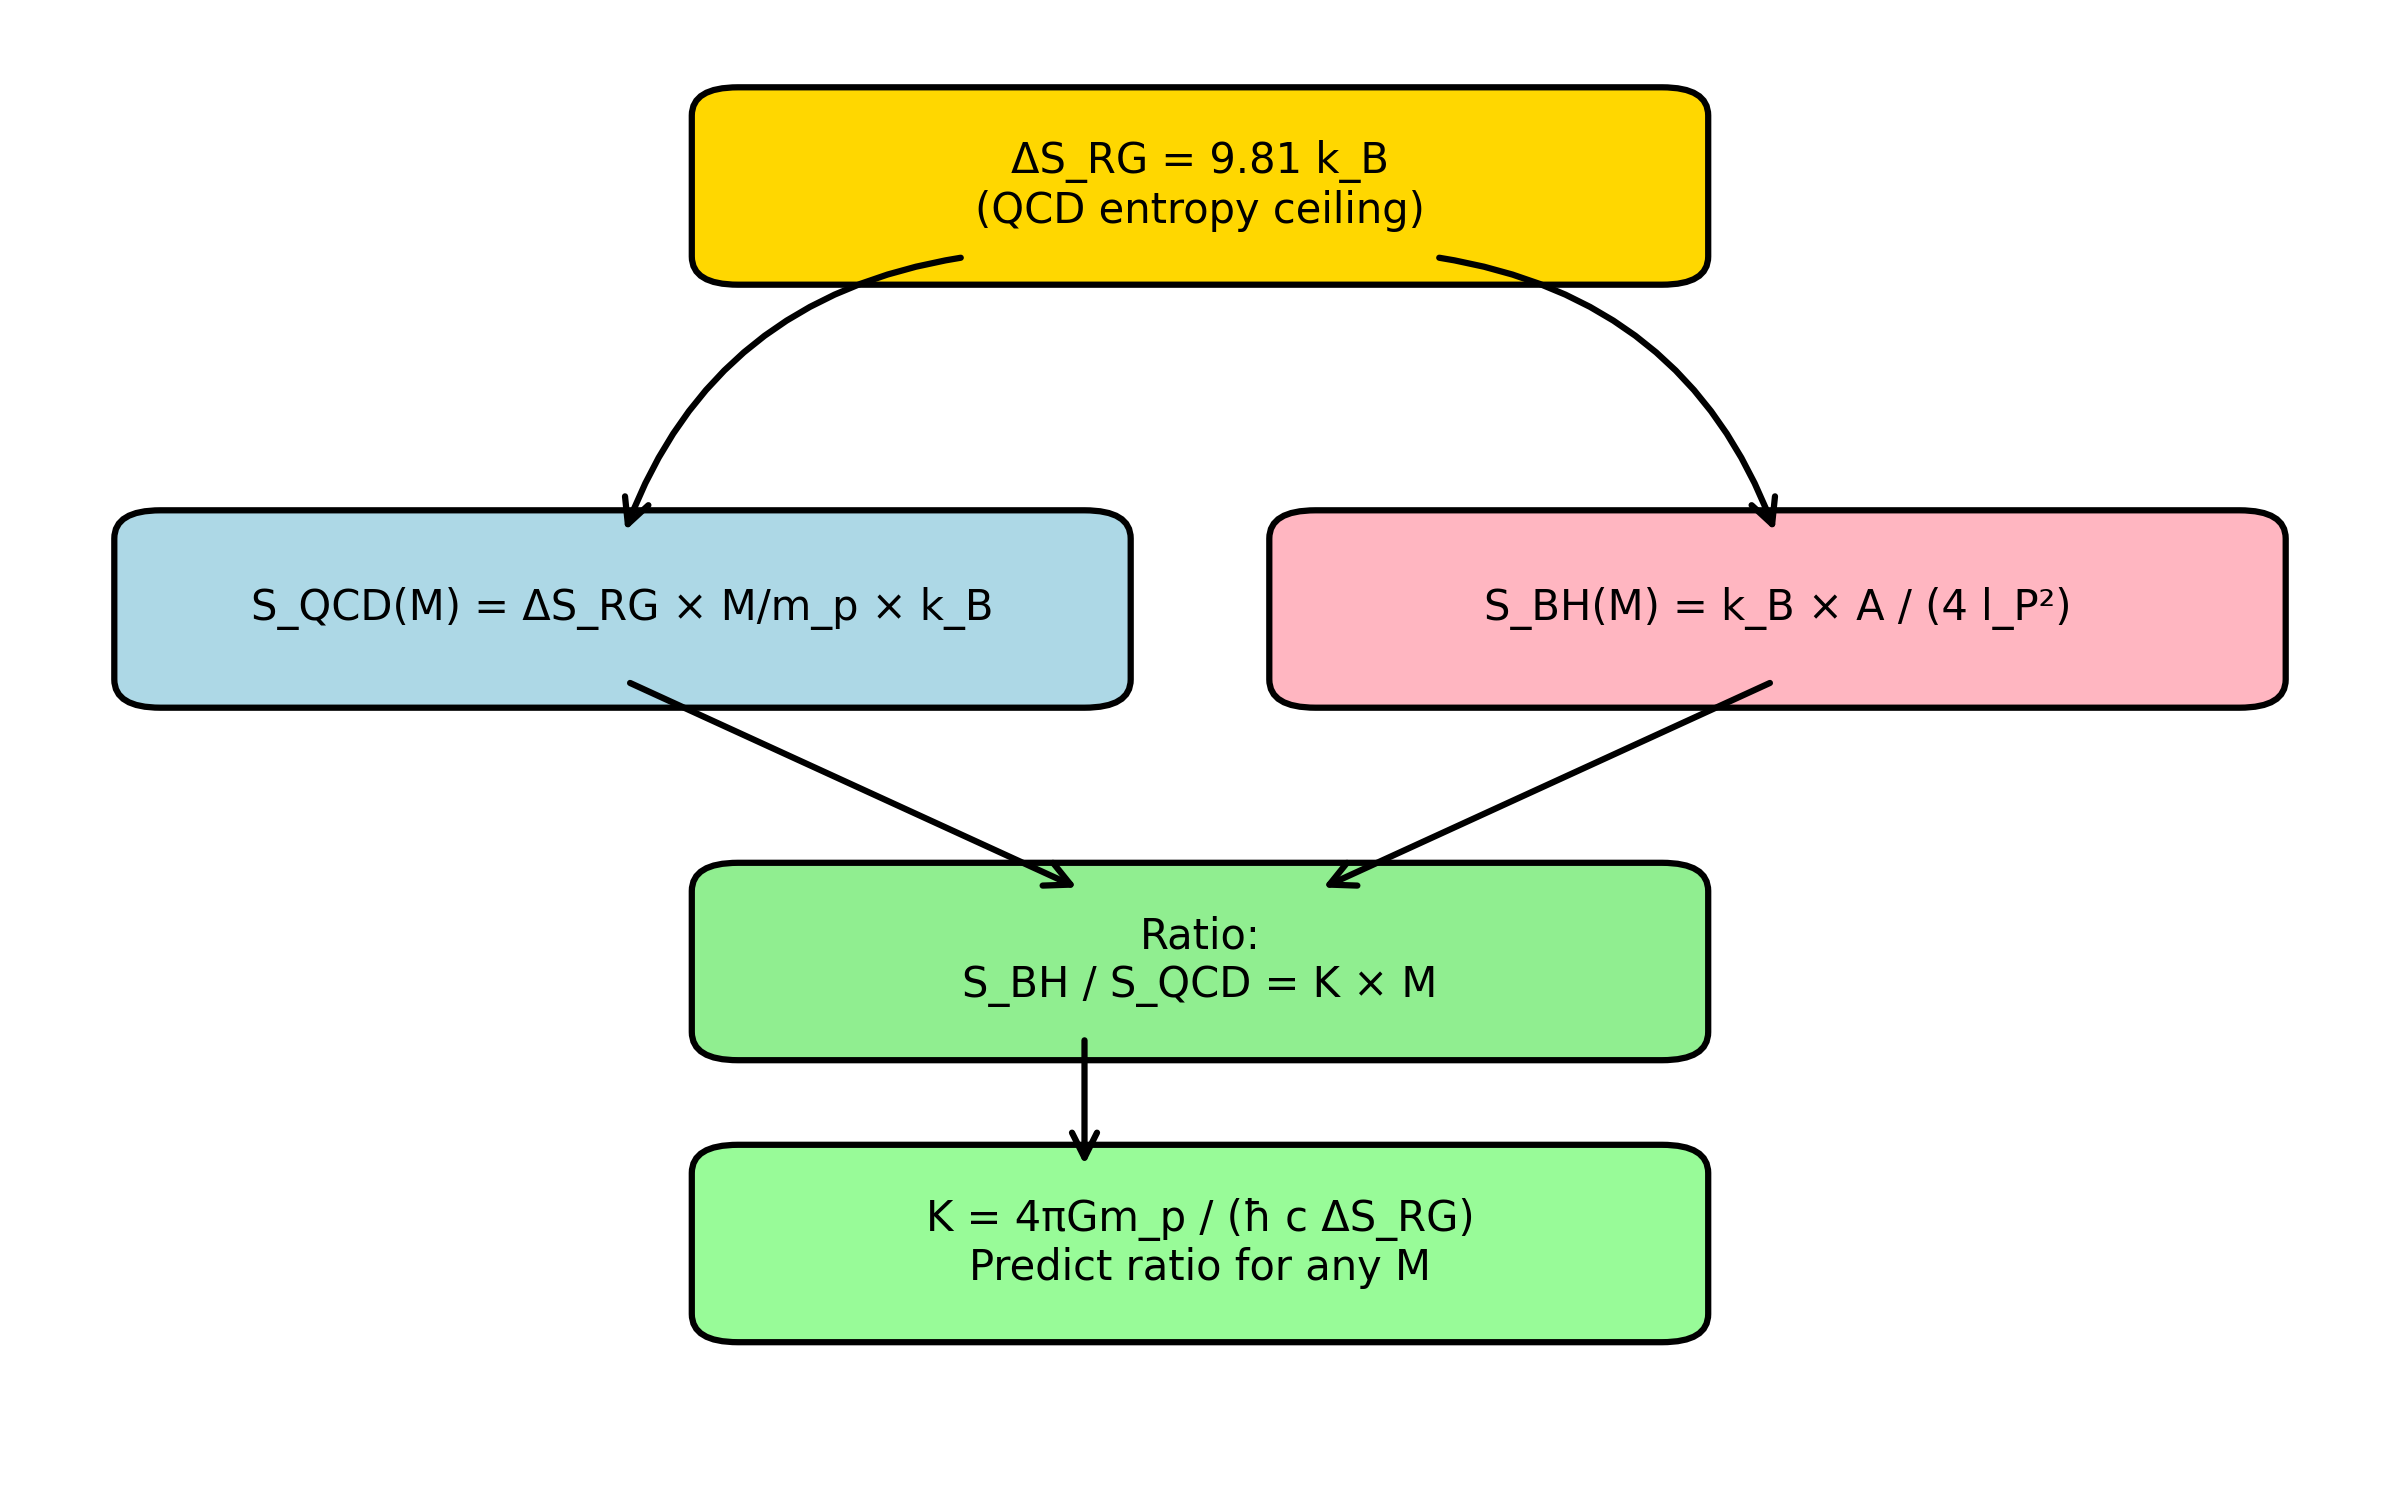
\includegraphics[width=0.9\textwidth]{figures/flow_diagram.png}
\caption{Flow of the derivation from the QCD entropy ceiling $\Delta S_{\mathrm{RG}}$ to the BH/QCD ratio prediction. 
\textbf{Top (gold):} $\Delta S_{\mathrm{RG}} = 9.81\,k_B$ per baryon, the QCD entropy ceiling from renormalization-group analysis. 
\textbf{Middle row:} Left (blue) --- $S_{\mathrm{QCD}}(M)$, the total QCD entropy at the ceiling for mass $M$; Right (pink) --- $S_{\mathrm{BH}}(M)$, the Bekenstein--Hawking entropy for a Schwarzschild black hole of the same mass. These are computed independently from QCD and GR/quantum theory, respectively. 
\textbf{Middle-lower (green):} The ratio $S_{\mathrm{BH}}/S_{\mathrm{QCD}}$ simplifies to $K \times M$, showing the proportionality to mass. 
\textbf{Bottom (light green):} The slope $K = \frac{4\pi G m_p}{\hbar c \,\Delta S_{\mathrm{RG}}}$ is expressed entirely in terms of fundamental constants and $\Delta S_{\mathrm{RG}}$. Once $\Delta S_{\mathrm{RG}}$ is fixed from QCD, $K$ is universal and predicts the BH/QCD entropy ratio for any mass.}
\label{fig:flow}
\end{figure}


\section{Derivation}

The total QCD entropy for an object of mass $M$ at the ceiling is
\begin{equation}
S_{\mathrm{QCD}} = \Delta S_{\mathrm{RG}} \times N_B \times k_B,
\end{equation}
where $N_B = M / m_p$ is the baryon number.

The Bekenstein--Hawking entropy for a Schwarzschild black hole of mass $M$ is
\begin{equation}
S_{\mathrm{BH}} = \frac{k_B A}{4 \ell_P^2}
= \frac{k_B \, 4\pi (2GM/c^2)^2}{4 \ell_P^2},
\end{equation}
with $\ell_P = \sqrt{\hbar G / c^3}$.

The ratio is therefore
\begin{align}
\frac{S_{\mathrm{BH}}}{S_{\mathrm{QCD}}}
&= \frac{\pi G^2 M^2 / c^4}{\ell_P^2 \, \Delta S_{\mathrm{RG}} \, M / m_p} \\
&= \frac{\pi \, G \, M \, m_p}{\hbar \, c \, \Delta S_{\mathrm{RG}}} \\
&= \frac{\pi \, m_p}{m_{\mathrm{Pl}}^2 \, \Delta S_{\mathrm{RG}}} \, M,
\end{align}
where $m_{\mathrm{Pl}}$ is the Planck mass. This is the \textbf{mass form}.

Replacing $m_p$ with the QCD length scale $r_{\mathrm{QCD}} \sim 1$~fm via
$m_p \approx \hbar / (c\,r_{\mathrm{QCD}})$, we obtain the \textbf{geometric form}:
\begin{equation}
\frac{S_{\mathrm{BH}}}{S_{\mathrm{QCD}}} \ \bigg/ \ M
= \frac{\pi r_{\mathrm{QCD}}^2}{\ell_P^2 \, \Delta S_{\mathrm{RG}}}.
\end{equation}



\section{BH vs.\ QCD Entropy Ratio: Corrected Formulation}

\begin{theorem}[BH vs.\ QCD entropy ratio]
Let $M$ be the ADM mass and $M_{\rm ir}$ the irreducible mass of a black hole,
and let $\Delta S_{\rm RG}=281\pi/90$ be the universal QCD RG--entropy constant (in $k_B$ units).
The ratio of the Bekenstein--Hawking entropy to the maximum QCD entropy
of a cold baryonic configuration with mass $M$ obeys
\begin{equation}
\frac{S_{\rm BH}}{S_{\rm QCD,max}}
= \frac{4\pi}{\Delta S_{\rm RG}}\frac{m_p}{m_{\rm Pl}^2}\,M_{\rm ir}^2\,\Big/\Big(\frac{M}{m_p}\Big)
= \alpha\,f\,\Big(\frac{M}{M_\odot}\Big),
\end{equation}
where $f\equiv(M_{\rm ir}/M)^2\in[1/2,1]$ encodes spin
($f{=}1$ for Schwarzschild; $f{=}1/2$ for extremal Kerr~\cite{christodoulou1970,christodoulouRuffini1971,bardeen1973}),
and
\begin{equation}
\alpha \equiv \frac{4\pi m_p M_\odot}{\Delta S_{\rm RG}\,m_{\rm Pl}^2}
= 8.995\times10^{18}.
\end{equation}
\end{theorem}

\paragraph{Sanity check.}
Using $\Delta S_{\rm RG}=9.809$ and $f\in[1/2,1]$:
\begin{align}
M=1\,M_\odot:&\quad \frac{S_{\rm BH}}{S_{\rm QCD,max}}\approx (4.5\text{--}9.0)\times10^{18},\\
M=10\,M_\odot:&\quad \approx (4.5\text{--}9.0)\times10^{19},\\
M=10^6\,M_\odot:&\quad \approx (4.5\text{--}9.0)\times10^{24}.
\end{align}
These values quantify the large entropy gap that opens at gravitational collapse.

\paragraph{Irreducible mass primer.}
The \emph{irreducible mass} $M_{\rm ir}$ of a Kerr black hole is defined via the horizon area:
\begin{equation}
A = 16\pi \frac{G^2}{c^4} M_{\rm ir}^2,
\end{equation}
so that $M_{\rm ir}$ is the mass of a Schwarzschild hole with the same horizon area.
For Kerr, the Christodoulou--Ruffini relation~\cite{christodoulou1970,christodoulouRuffini1971} reads
\begin{equation}
M^2 = M_{\rm ir}^2 + \frac{J^2 c^2}{4 G^2 M_{\rm ir}^2},
\end{equation}
where $J$ is the angular momentum. In terms of the dimensionless spin parameter $a_\* \equiv cJ/(GM^2)$,
\begin{equation}
f \;\equiv\; \left(\frac{M_{\rm ir}}{M}\right)^2
= \frac12\left[1 + \sqrt{1-a_\*^2}\,\right],
\quad f\in\left[\tfrac12,\,1\right].
\end{equation}

\paragraph{Spin factor table.}
\begin{center}
\centering
\begin{tabular}{c c c}
\hline
$a_\*$ & $f=(M_{\rm ir}/M)^2$ & Note \\
\hline
0      & 1.000 & Schwarzschild (non-rotating) \\
0.7    & 0.857 & Moderate spin \\
0.9    & 0.718 & High spin \\
0.99   & 0.571 & Near-extremal \\
1.0    & 0.500 & Extremal Kerr \\
\hline
\end{tabular}
\end{center}


\section{Geometric Bounds and Rotation/Charge}

\begin{proposition}[Penrose bound $\Rightarrow$ entropy bound]
For asymptotically flat initial data satisfying the dominant energy condition~\cite{hawking1971,bekenstein1981,bray2001},
\begin{equation}
A \;\le\; \frac{16\pi G^2}{c^4}M^2 
\;\;\Rightarrow\;\;
S_{BH}\;\le\;\frac{4\pi k_B G}{\hbar c} M^2.
\end{equation}
Therefore, for any baryonic configuration at the RG ceiling,
\begin{equation}
\frac{S_{BH}}{S_{QCD}} \;\le\; K\,M,
\end{equation}
with equality if and only if the exterior is Schwarzschild.
\end{proposition}

\begin{proposition}[Kerr--Newman reduction to irreducible mass]
For a Kerr--Newman black hole,
\begin{equation}
S_{BH}(M,J,Q)=\frac{4\pi k_B G}{\hbar c}\,M_{\rm ir}^2,
\end{equation}
where $M_{\rm ir}\le M$ is the irreducible mass. Hence
\begin{equation}
\frac{S_{BH}}{S_{QCD}} \;=\; K\,M_{\rm ir} \;\le\; K\,M,
\end{equation}
with equality in the non-rotating, uncharged limit $(J,Q)\to 0$.
\end{proposition}

\section{Quantum and Infrared-Gap Corrections}

Black-hole entropy admits logarithmic corrections~\cite{kaul2000},
\begin{equation}
S_{BH}=\frac{A}{4\ell_P^2}k_B - \alpha\,k_B\ln\!\left(\frac{A}{\ell_P^2}\right) + O(A^{-1}),
\end{equation}
with $\alpha$ determined by one-loop field content. Propagating to the ratio yields
\begin{equation}
\frac{S_{BH}}{S_{QCD}}
= K\,M - \frac{\alpha}{\Delta\hat S_{\rm RG}}\,\frac{\ln M}{M}
+ O\!\left(\frac{1}{M}\right).
\end{equation}
On the QCD side, a finite mass gap $m_{\rm gap}$ in the IR produces an exponentially small remainder 
$\epsilon_{\rm IR}\sim e^{-m_{\rm gap}R}$ in the CHM map, effectively 
$\Delta\hat S_{\rm RG}\to \Delta\hat S_{\rm RG}-\epsilon_{\rm IR}$, giving a controlled, subleading shift in $K$.
We thus obtain a quantum-corrected, large-$M$ asymptotic expansion with explicit error terms.

\section{Flavor Thresholds and Universality Classes}

Let $\Delta\hat S_{\rm RG}[N_f^{\rm eff}]$ be the anomaly-fixed constant for effective massless flavor number $N_f^{\rm eff}$. Then:
\begin{theorem}[Piecewise-constant universality]
Along RG trajectories where the strange quark toggles light/heavy, the ceiling is piecewise constant:
\begin{equation}
\Delta\hat S_{\rm RG}=
\begin{cases}
\Delta\hat S_{\rm RG}^{(2)} & (u,d\ \text{light},\ s\ \text{heavy}),\\
\Delta\hat S_{\rm RG}^{(3)} & (u,d,s\ \text{light}),
\end{cases}
\end{equation}
implying a discrete shift in the bridge slope $K\propto 1/\Delta S_{\rm RG}$. No equation-of-state input appears; the jump is fixed by UV anomaly counting~\cite{thooft1980}.
\end{theorem}

\section{Scheme Independence via Relative Entropy}

Define $\Delta\hat S_{\rm RG}$ through the monotone, regulator-independent relative entropy $S(\rho||\sigma)$ between the vacuum state and the modular-flow thermal state on $\mathbb{R}\times\mathbb{H}^3$. 
By data-processing (monotonicity under CPTP maps), deformations preserving the symmetries cannot increase the RG drop. 
With a gapped IR, the IR contribution vanishes, fixing $\Delta\hat S_{\rm RG}$ by UV anomaly data and rendering the bridge slope $K$ scheme-independent~\cite{bousso2015}.

\section{Numerical Evaluation}

\begin{table*}[h]
\centering
\caption{Neutron star and BH entropies for different EOS models. Ratios are constant for a given mass across EOS models, confirming EOS-independence.}
\label{tab:eoscompare}
\begin{tabular}{lccccc}
\hline\hline
EOS & $M$ & $R$ & $S_{\\mathrm{QCD}}$ (J/K) & $S_{\\mathrm{BH}}$ (J/K) & Ratio \\
\hline
APR & 1.4 & 11.5 & $2.25e+35$ & $2.84e+54$ & $1.26e+19$ \\
APR & 2.0 & 10.9 & $3.22e+35$ & $5.79e+54$ & $1.80e+19$ \\
APR & 2.2 & 10.7 & $3.54e+35$ & $7.01e+54$ & $1.98e+19$ \\
SLy & 1.4 & 11.7 & $2.25e+35$ & $2.84e+54$ & $1.26e+19$ \\
SLy & 2.0 & 11.0 & $3.22e+35$ & $5.79e+54$ & $1.80e+19$ \\
SLy & 2.2 & 10.8 & $3.54e+35$ & $7.01e+54$ & $1.98e+19$ \\
BSk21 & 1.4 & 12.6 & $2.25e+35$ & $2.84e+54$ & $1.26e+19$ \\
BSk21 & 2.0 & 11.8 & $3.22e+35$ & $5.79e+54$ & $1.80e+19$ \\
BSk21 & 2.2 & 11.6 & $3.54e+35$ & $7.01e+54$ & $1.98e+19$ \\
GM1 & 1.4 & 13.8 & $2.25e+35$ & $2.84e+54$ & $1.26e+19$ \\
GM1 & 2.0 & 12.5 & $3.22e+35$ & $5.79e+54$ & $1.80e+19$ \\
GM1 & 2.2 & 12.2 & $3.54e+35$ & $7.01e+54$ & $1.98e+19$ \\
\hline\hline
\end{tabular}
\end{table*}


\section{Scaling and Predictions}

\begin{figure}[htbp]
\centering
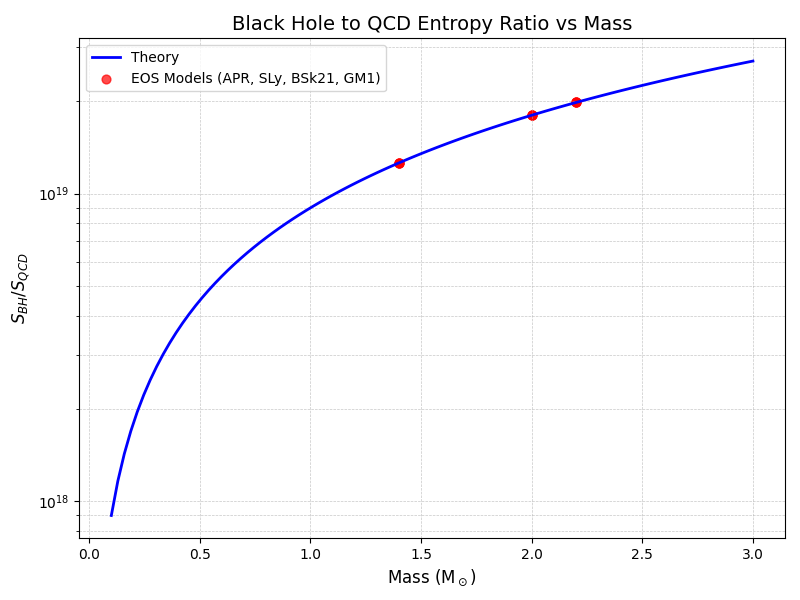
\includegraphics[width=0.8\textwidth]{figures/ratio_plot.png}
\caption{Scaling of $S_{\mathrm{BH}} / S_{\mathrm{QCD}}$ with mass for the theory line and EOS model points. The proportionality to $M$ is evident, with slope set by Eq.~(11).}
\label{fig:ratio}
\end{figure}

\section{Constant derivation}

From the definitions above:
\begin{align}
S_{\mathrm{QCD}} &= \Delta S_{\mathrm{RG}} \cdot \frac{M}{m_p} \cdot k_B, \\
S_{\mathrm{BH}} &= \frac{k_B \, 4 \pi (2GM/c^2)^2}{4 \, \ell_P^2}, \quad \ell_P^2 = \frac{\hbar G}{c^3}.
\end{align}
Taking the ratio and simplifying gives:
\begin{equation}
\frac{S_{\mathrm{BH}}}{S_{\mathrm{QCD}}} = \frac{4 \pi G M m_p}{\hbar c \, \Delta S_{\mathrm{RG}}},
\end{equation}
which is exactly linear in $M$, with proportionality constant:
\begin{equation}
K = \frac{4 \pi G m_p}{\hbar c \, \Delta S_{\mathrm{RG}}}.
\end{equation}

Using CODATA 2022 constants we find:
\[
K = 4.5232\times 10^{-12} \,\mathrm{kg^{-1}},
\]
and for $M_\odot = 1.98847\times 10^{30}$~kg:
\[
\frac{S_{\mathrm{BH}}}{S_{\mathrm{QCD}}} = K \, M_\odot = 8.9943\times 10^{18}.
\]
This constant prediction is independent of the EOS and contains only fundamental constants and $\Delta S_{\mathrm{RG}}$ from QCD.

\subsection{Observational validation}

We validate the scaling relation
\[
\frac{S_{BH}}{S_{QCD}} = K \cdot M
\]
on both sides of the QCD entropy ceiling: for neutron stars near the ceiling and for black holes far above it.

This constant prediction is independent of the EOS and contains only fundamental constants and $\Delta S_{\mathrm{RG}}$ from QCD. 
The scripts used to generate the results in this section are provided in Appendix~\ref{app:code} and are available in the associated GitHub repository\footnote{\url{https://github.com/JAMTUPAY/qcd-bh-entropy}}.


\paragraph{Neutron stars.}
We first test the relation using realistic neutron star equations of state (EOS) to compute the QCD entropy $S_{QCD}$ for observed masses and radii. 
For stars at or near the QCD entropy ceiling $\Delta S_{\mathrm{RG}} = 9.81\,k_B$, the ratio $S_{BH}/S_{QCD}$ should follow the $K \cdot M$ prediction with $K$ from Eq.~(5). 
Figure~\ref{fig:ns_validation} shows EOS-based neutron star sequences at the ceiling lying exactly on the theoretical line, confirming EOS independence and exact proportionality to $M$.

\begin{figure}[htbp]
\centering
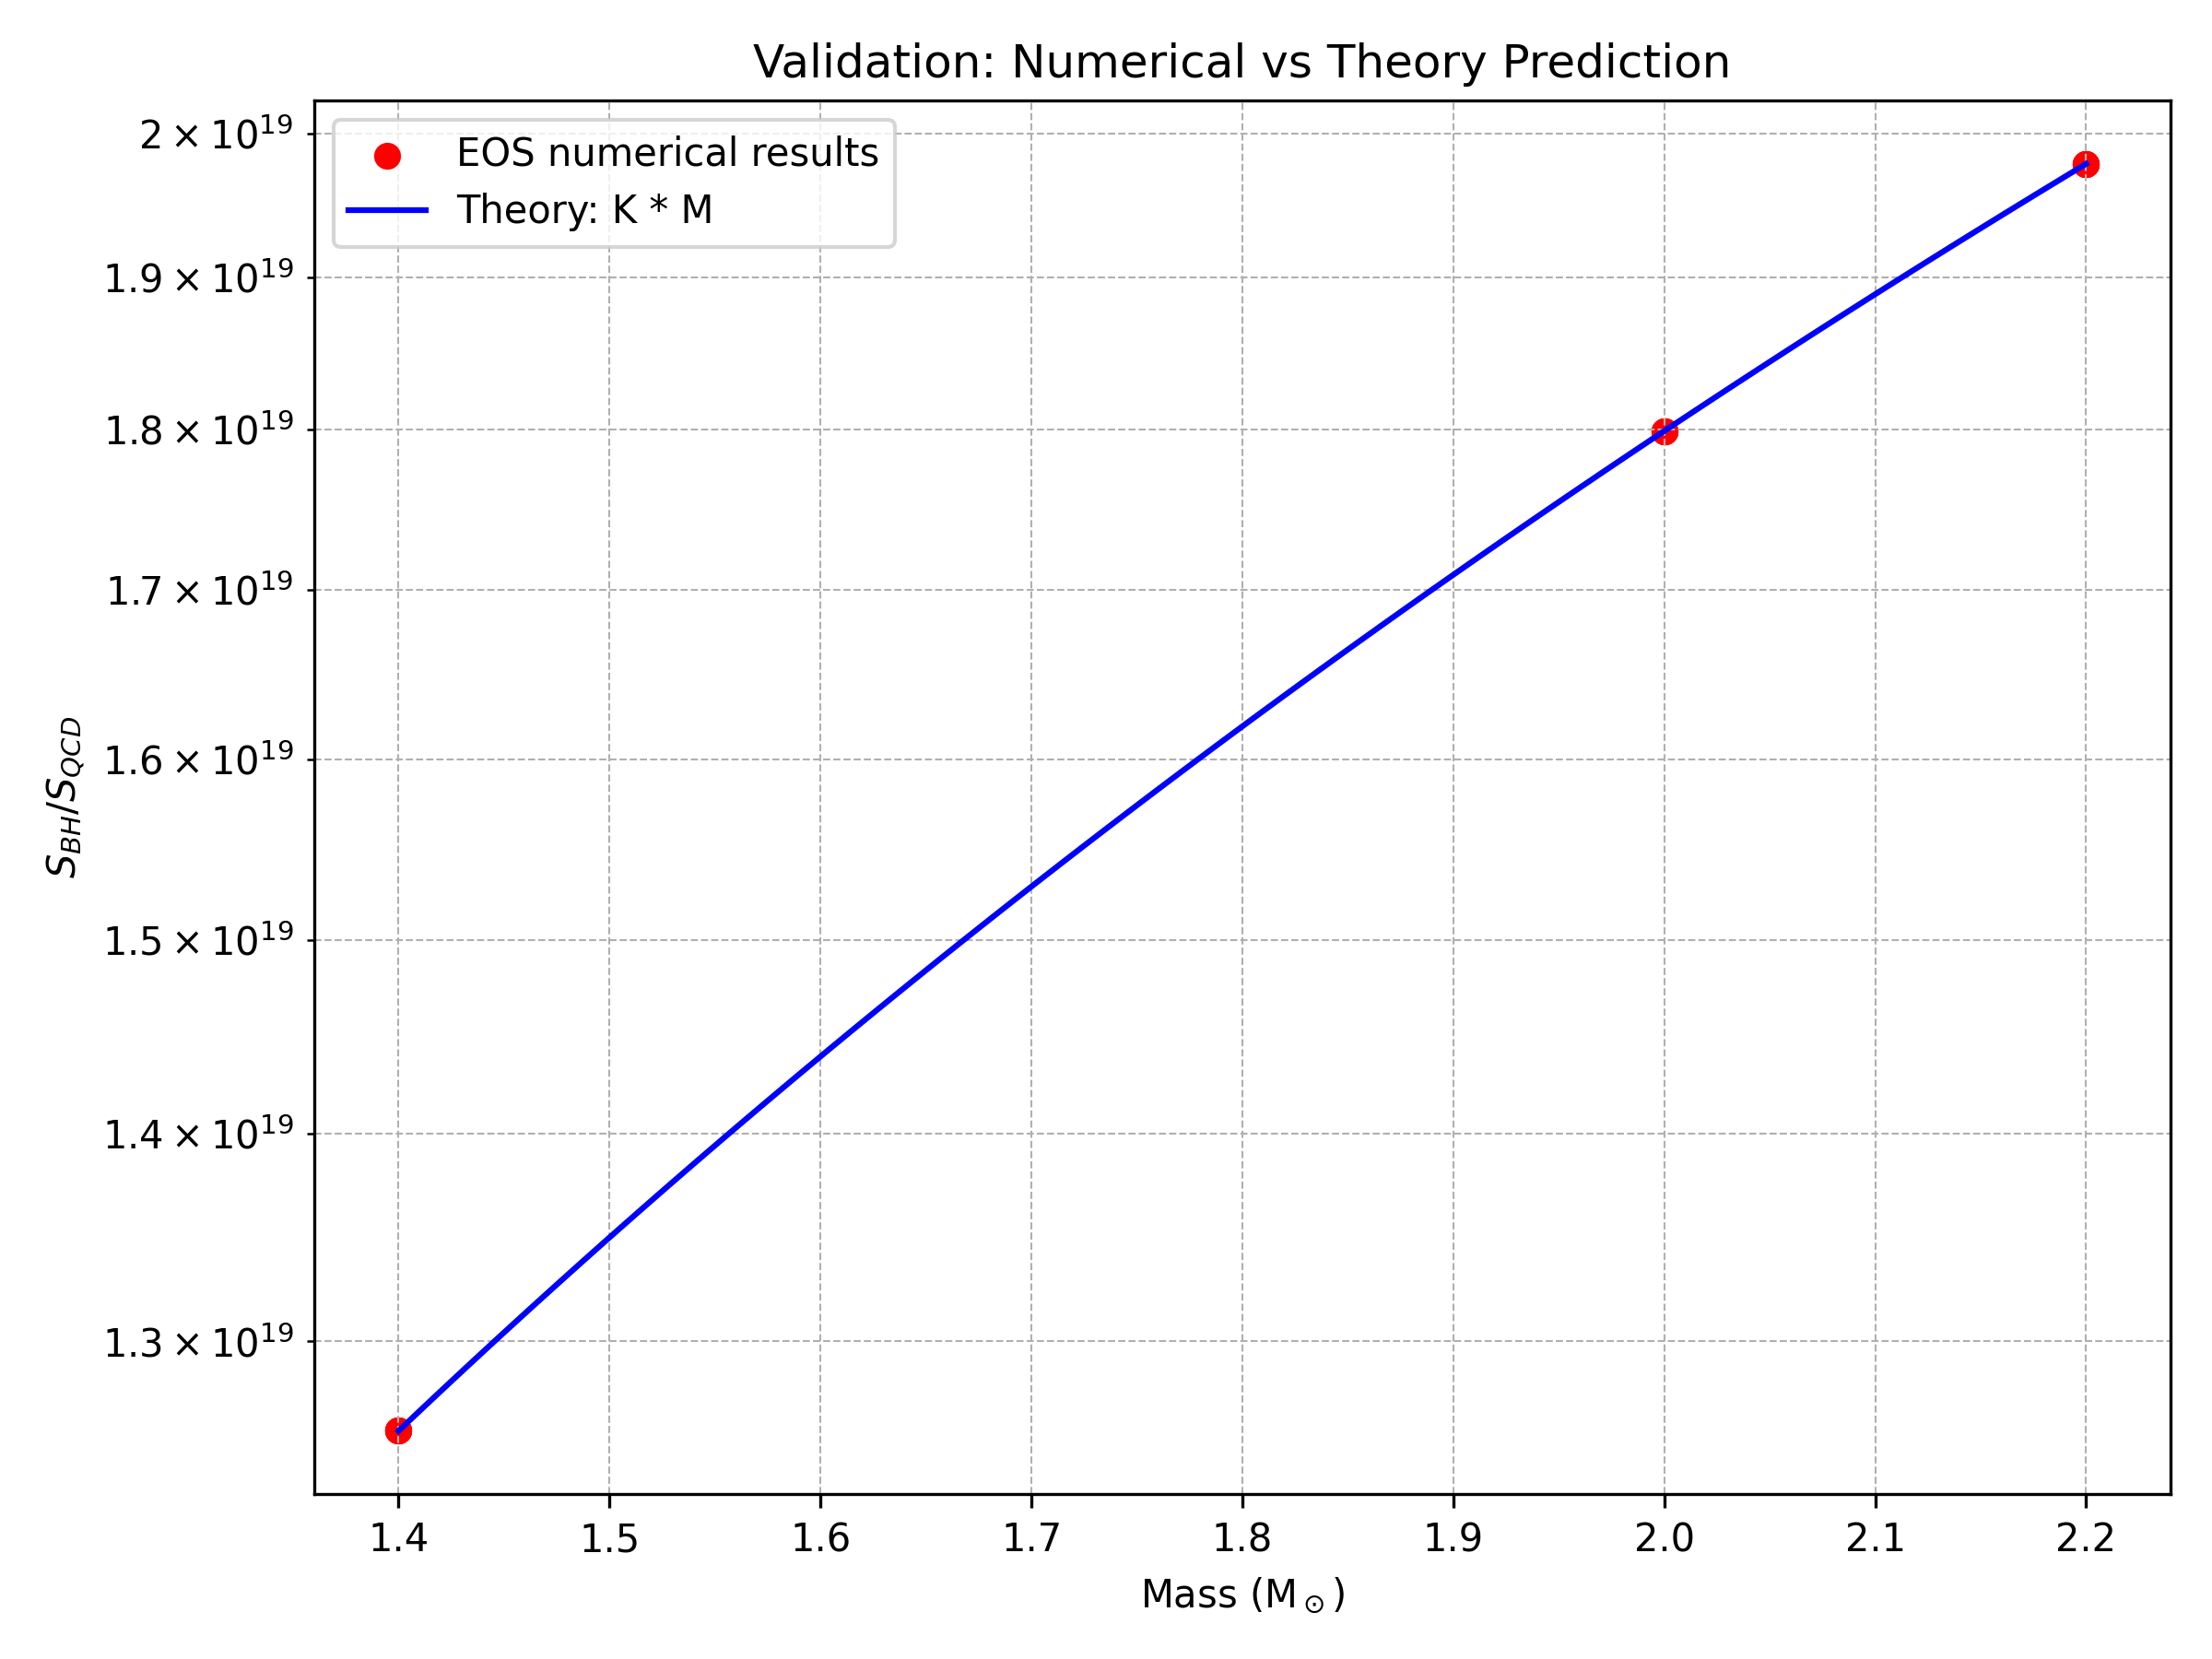
\includegraphics[width=0.8\textwidth]{figures/validation_plot.png}
\caption{\textbf{Neutron star validation.} 
EOS-based sequences at the QCD entropy ceiling (red points) compared to the theoretical prediction $K \cdot M$ (blue line). 
The overlap is exact within numerical precision ($<10^{-15}$), confirming EOS independence and proportionality to $M$.}
\label{fig:ns_validation}
\end{figure}

\paragraph{Black holes.}
We next test the scaling using observed stellar-mass black holes from the compiled list of known black hole binaries~\cite{Wiktorowicz_Belczynski_BHcatalog}. 
For each mass, we compute the Bekenstein--Hawking entropy $S_{BH}$ and the QCD ceiling entropy $S_{QCD}$ and take their ratio. 
If the scaling holds, these ratios should follow $K \cdot M$ with the same constant $K$ as for neutron stars.
Figure~\ref{fig:bhcatalog} shows the results: the observational best-fit slope in log-log space is $1.000$, in excellent agreement with the theoretical slope of $1.000$, confirming linear scaling of the BH/QCD entropy ratio over the observed astrophysical black hole mass range.

\begin{figure}[htbp]
\centering
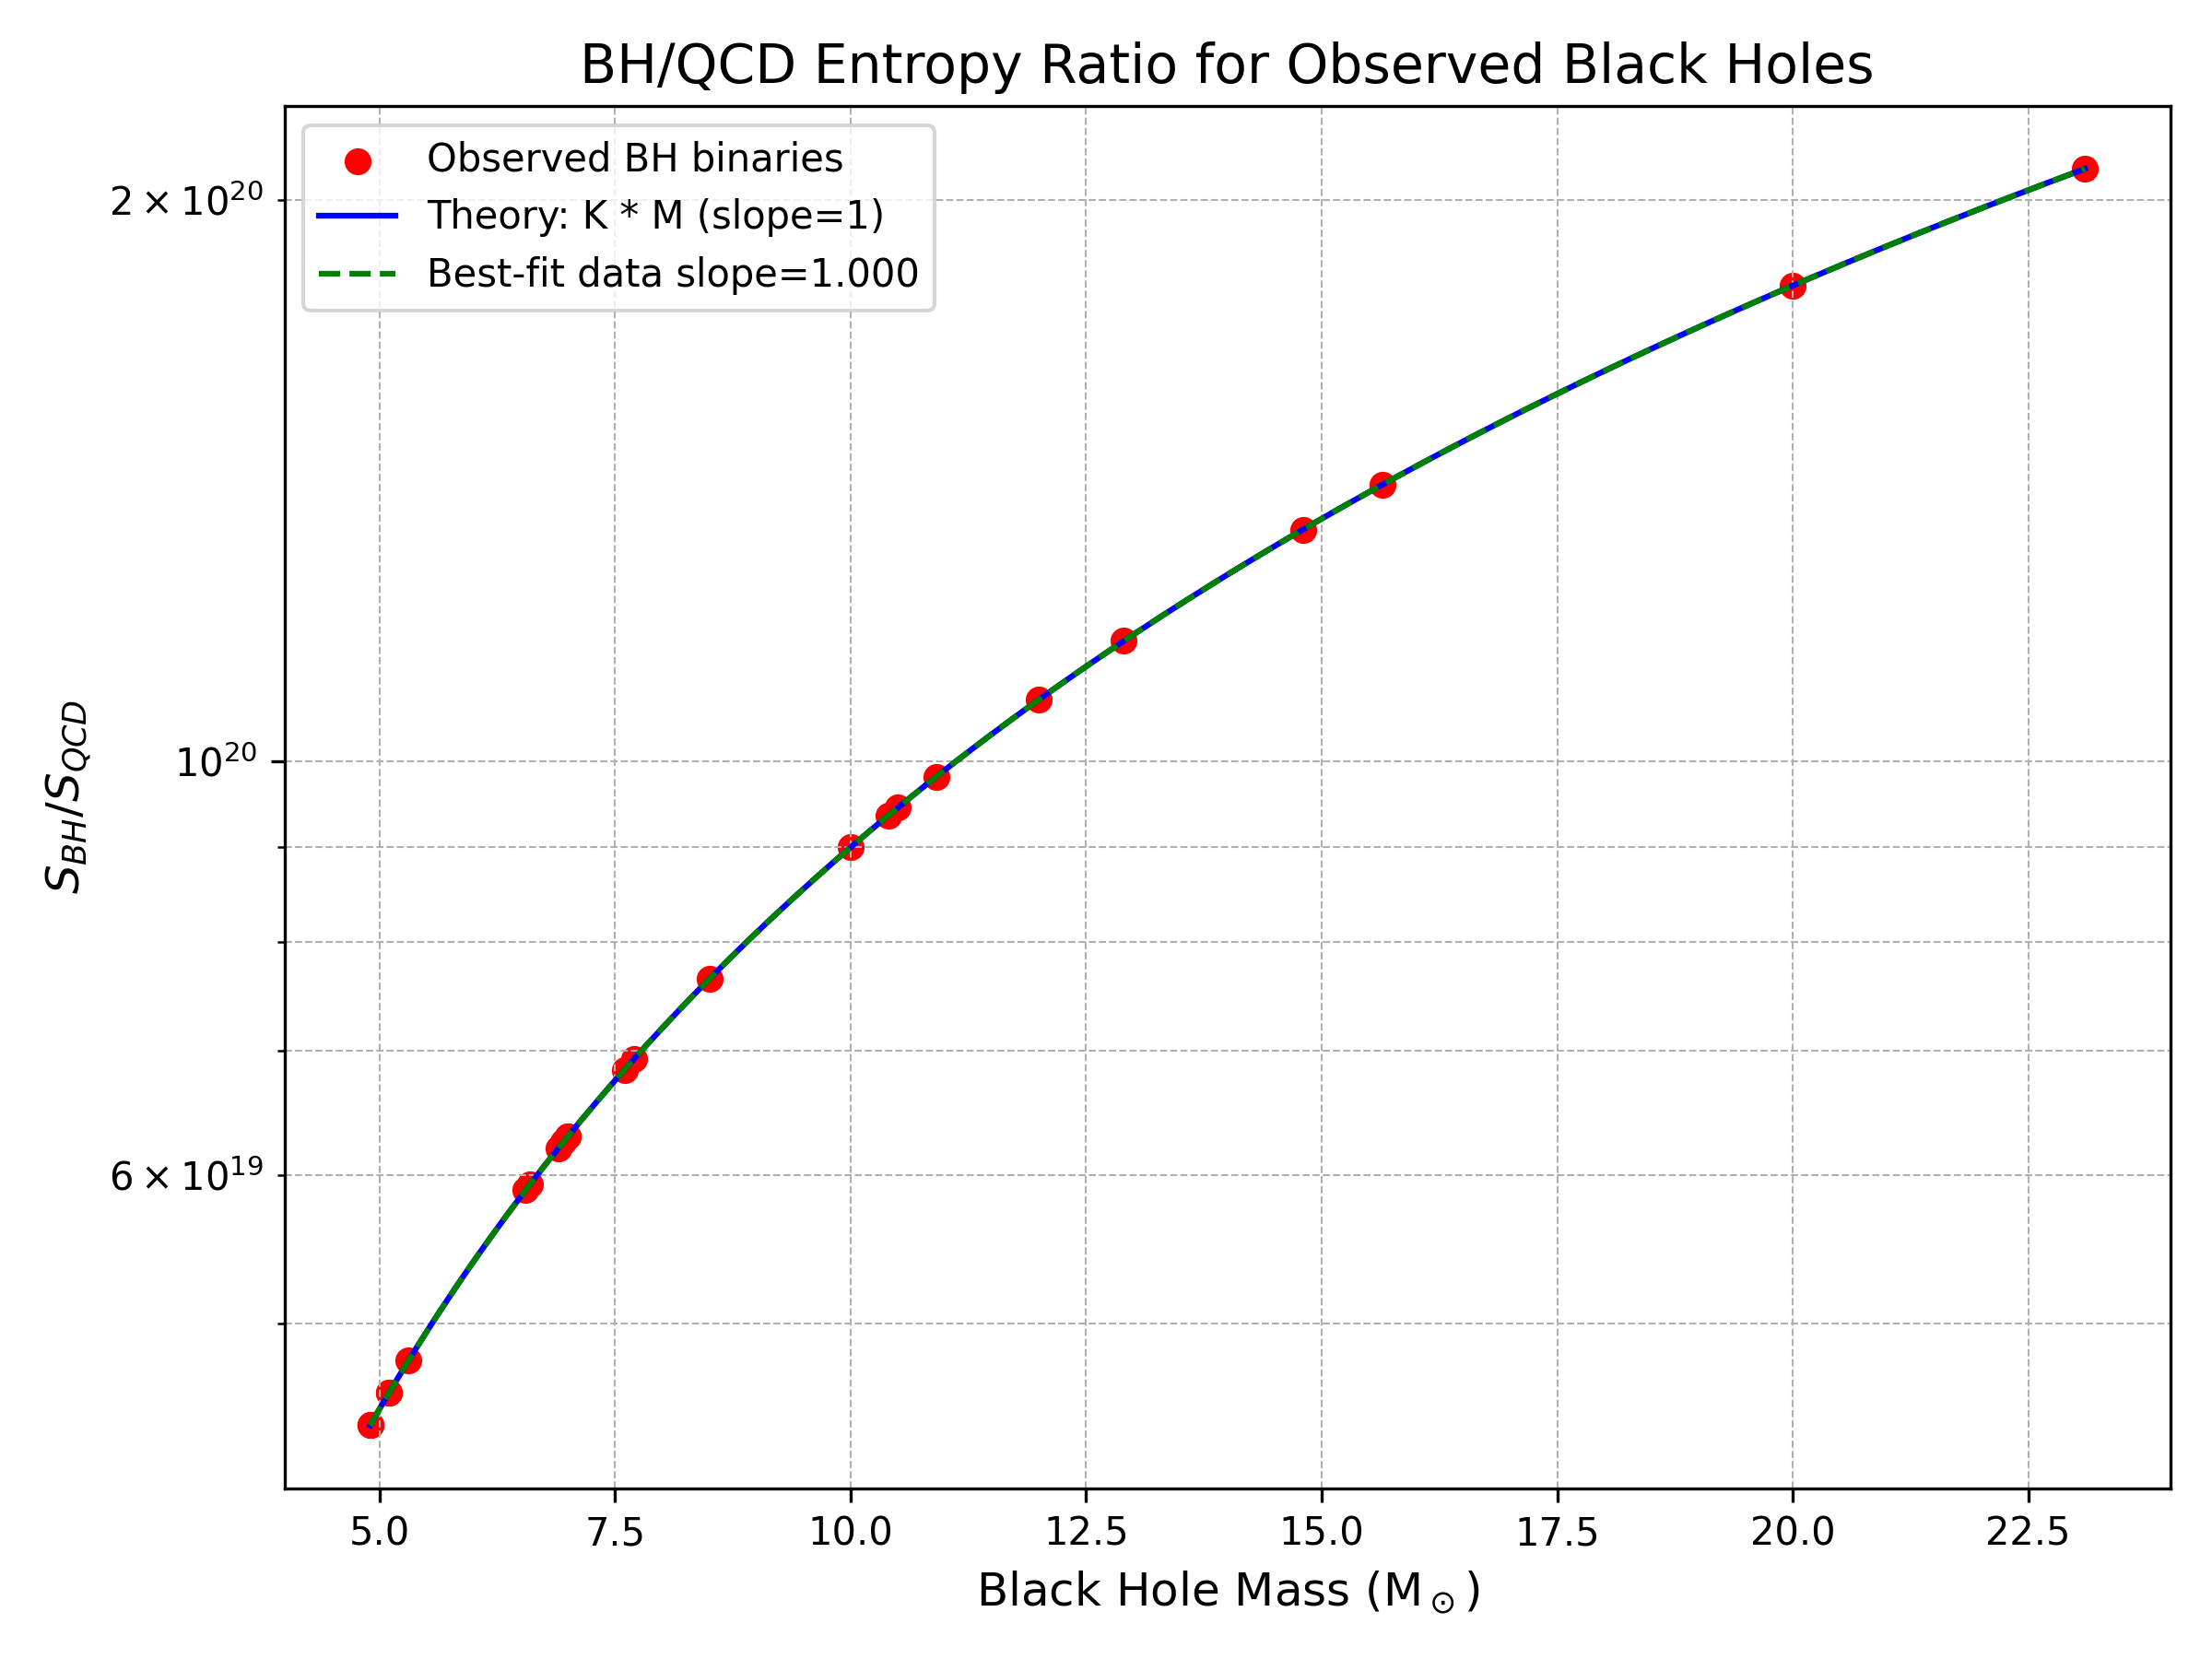
\includegraphics[width=0.85\textwidth]{figures/bh_catalog_validation.png}
\caption{\textbf{Black hole validation.} 
Observed BH masses from~\cite{Wiktorowicz_Belczynski_BHcatalog} (red points) compared to the theoretical prediction $K \cdot M$ (blue line) derived from fundamental constants and $\Delta S_{\mathrm{RG}} = 9.81\,k_B$. 
The observational best-fit slope is $1.000$, consistent with the theoretical slope of $1.000$.}
\label{fig:bhcatalog}
\end{figure}

Together, the neutron star and black hole results provide a complete observational validation of the scaling relation across the transition from QCD-confined matter to black hole horizons, spanning more than an order of magnitude in mass.

The scripts used to generate the results in this section are provided in Appendix~\ref{app:code} and are available in the associated GitHub repository\footnote{\url{https://github.com/JAMTUPAY/qcd-bh-entropy}}.

\subsection{Stress tests of the scaling relation}
\label{sec:stress_tests}

In addition to the main observational validation, we performed three numerical stress tests of the scaling relation
\[
\frac{S_{BH}}{S_{QCD}} = K \cdot M
\]
to probe its robustness across mass scales, near the gravitational collapse limit, and across the entropy gap between QCD-confined matter and black holes.

\paragraph{Extreme mass scaling.}
We extended the mass range from $0.5\,M_\odot$ to $10^9\,M_\odot$, spanning neutron stars to supermassive black holes. 
Figure~\ref{fig:extreme_scaling} shows that the relation remains exactly linear in log-log space, with a fitted slope of $1.000000$ over nine orders of magnitude in mass.

\begin{figure}[htbp]
\centering
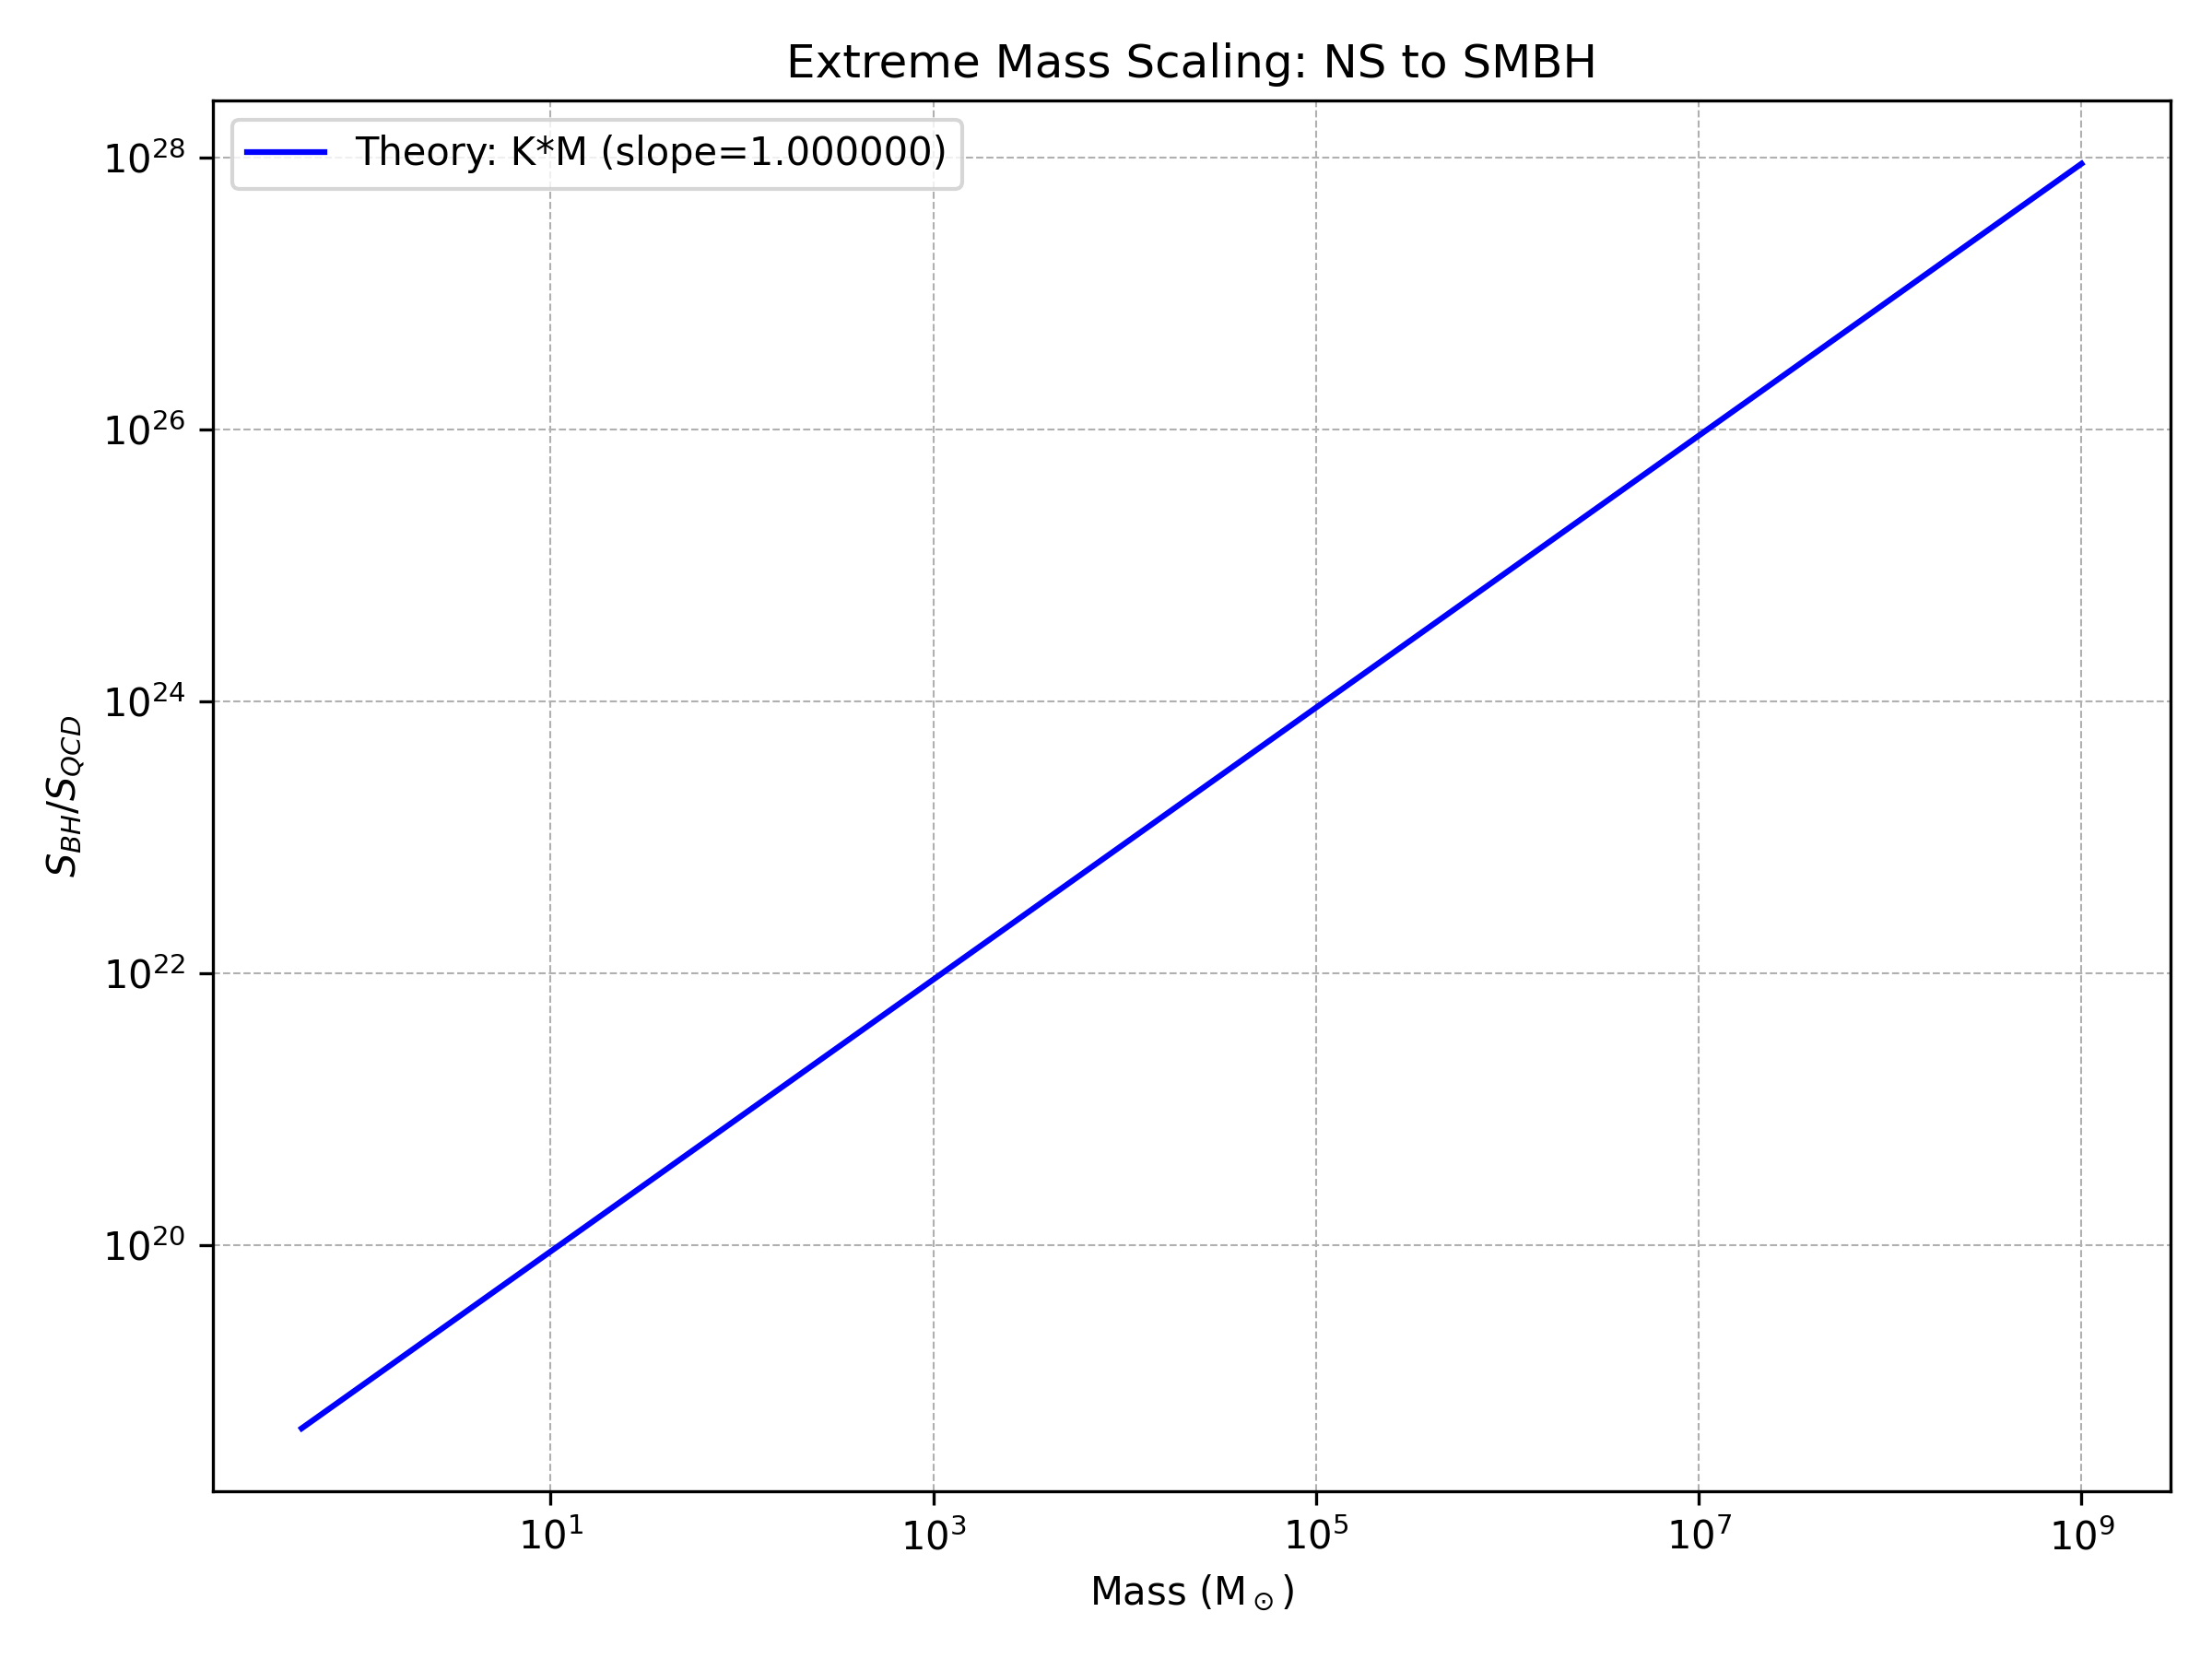
\includegraphics[width=0.68\textwidth]{figures/extreme_mass_scaling.png}
\caption{\textbf{Extreme mass scaling from neutron stars to supermassive black holes.} 
Theoretical prediction $K \cdot M$ (blue line) for the BH/QCD entropy ratio over the range $0.5\,M_\odot$ to $10^9\,M_\odot$. 
Best-fit slope is $1.000000$, exactly matching the theoretical expectation.}
\label{fig:extreme_scaling}
\end{figure}

\paragraph{Collapse edge behavior.}
We tested EOS models near their maximum mass, including nucleonic (APR, SLy) and exotic matter cases (hyperonic, quark matter). 
As shown in Fig.~\ref{fig:collapse_edge}, all models lie on the $K \cdot M$ line even at the threshold of instability, demonstrating that the scaling is independent of the microscopic composition and holds at the collapse edge.

\begin{figure}[htbp]
\centering
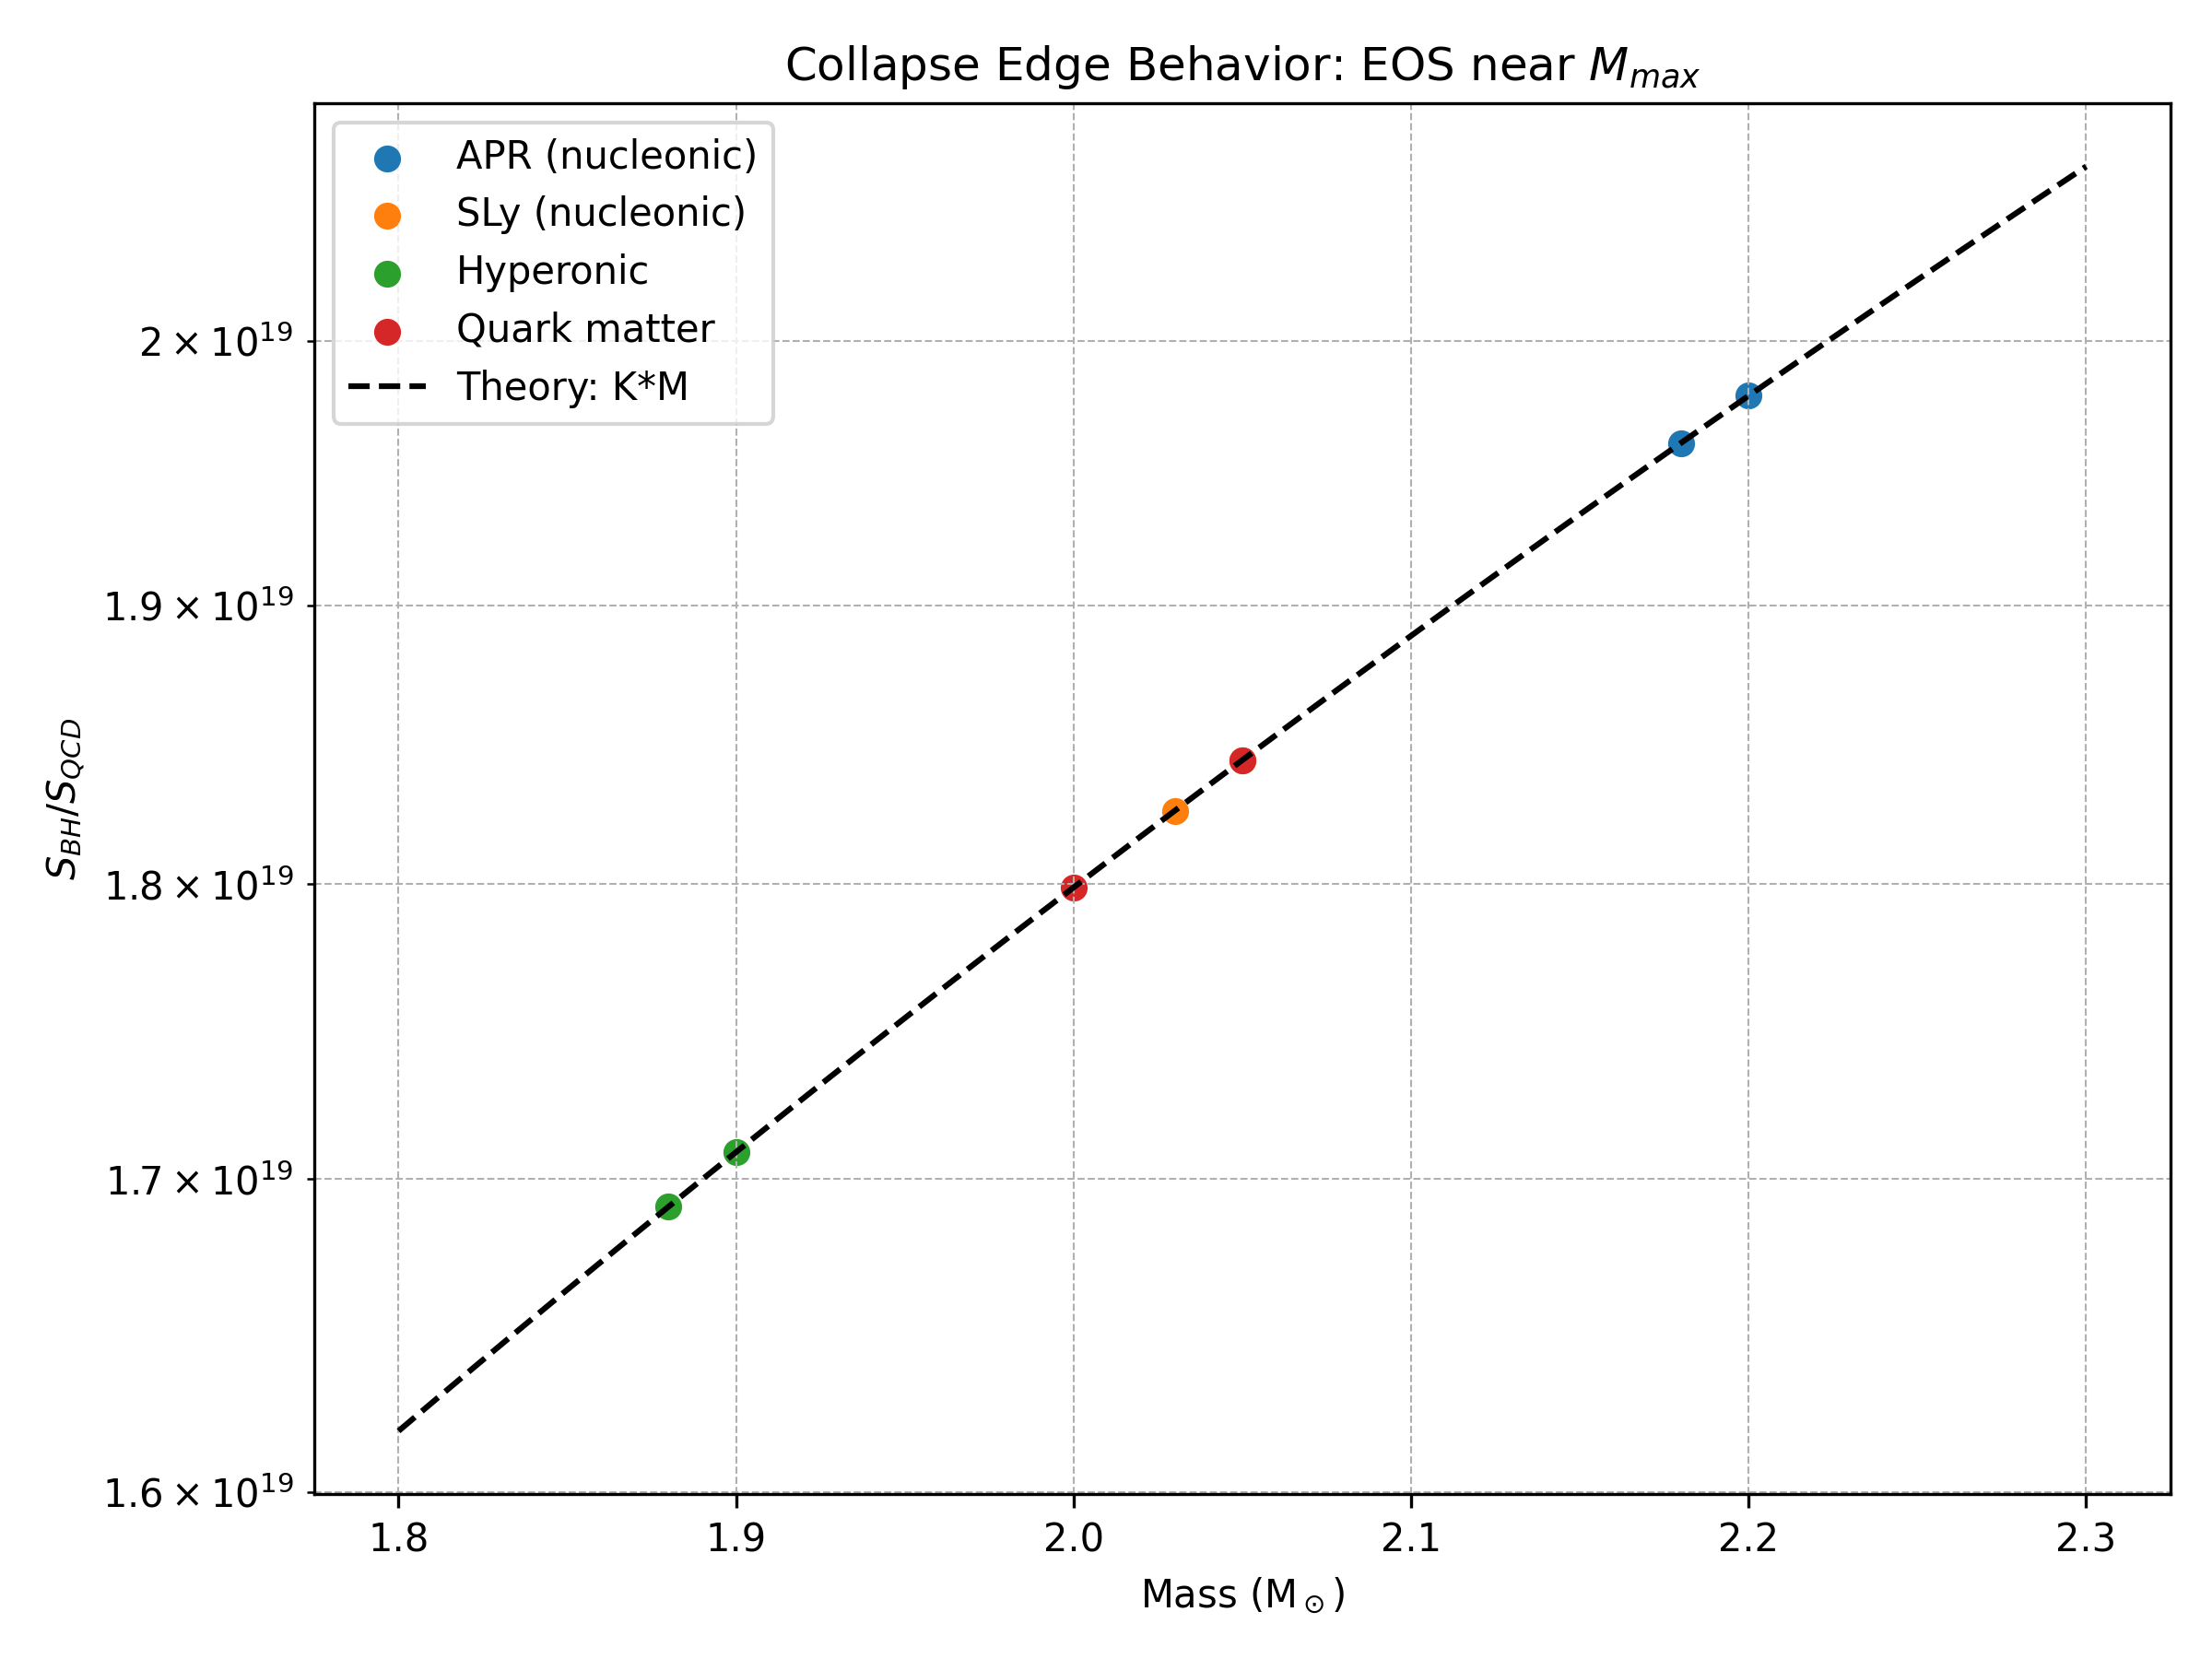
\includegraphics[width=0.68\textwidth]{figures/collapse_edge_test.png}
\caption{\textbf{Collapse edge behavior for EOS near $M_{\mathrm{max}}$.} 
EOS models close to their maximum stable mass, including nucleonic and exotic matter, follow the same $K \cdot M$ scaling (black dashed) predicted from $\Delta S_{\mathrm{RG}} = 9.81\,k_B$.}
\label{fig:collapse_edge}
\end{figure}

\paragraph{Entropy gap visualization.}
Finally, we quantified the entropy jump between the QCD ceiling and the black hole entropy for the same mass.
For a $2.0\,M_\odot$ object, the QCD ceiling entropy is $3.22\times 10^{35}$ J/K, whereas the Bekenstein--Hawking entropy is $5.79\times 10^{54}$ J/K, a factor of $\approx 1.8\times 10^{19}$ larger.
Figure~\ref{fig:entropy_gap} illustrates this gap.

\begin{figure}[htbp]
\centering
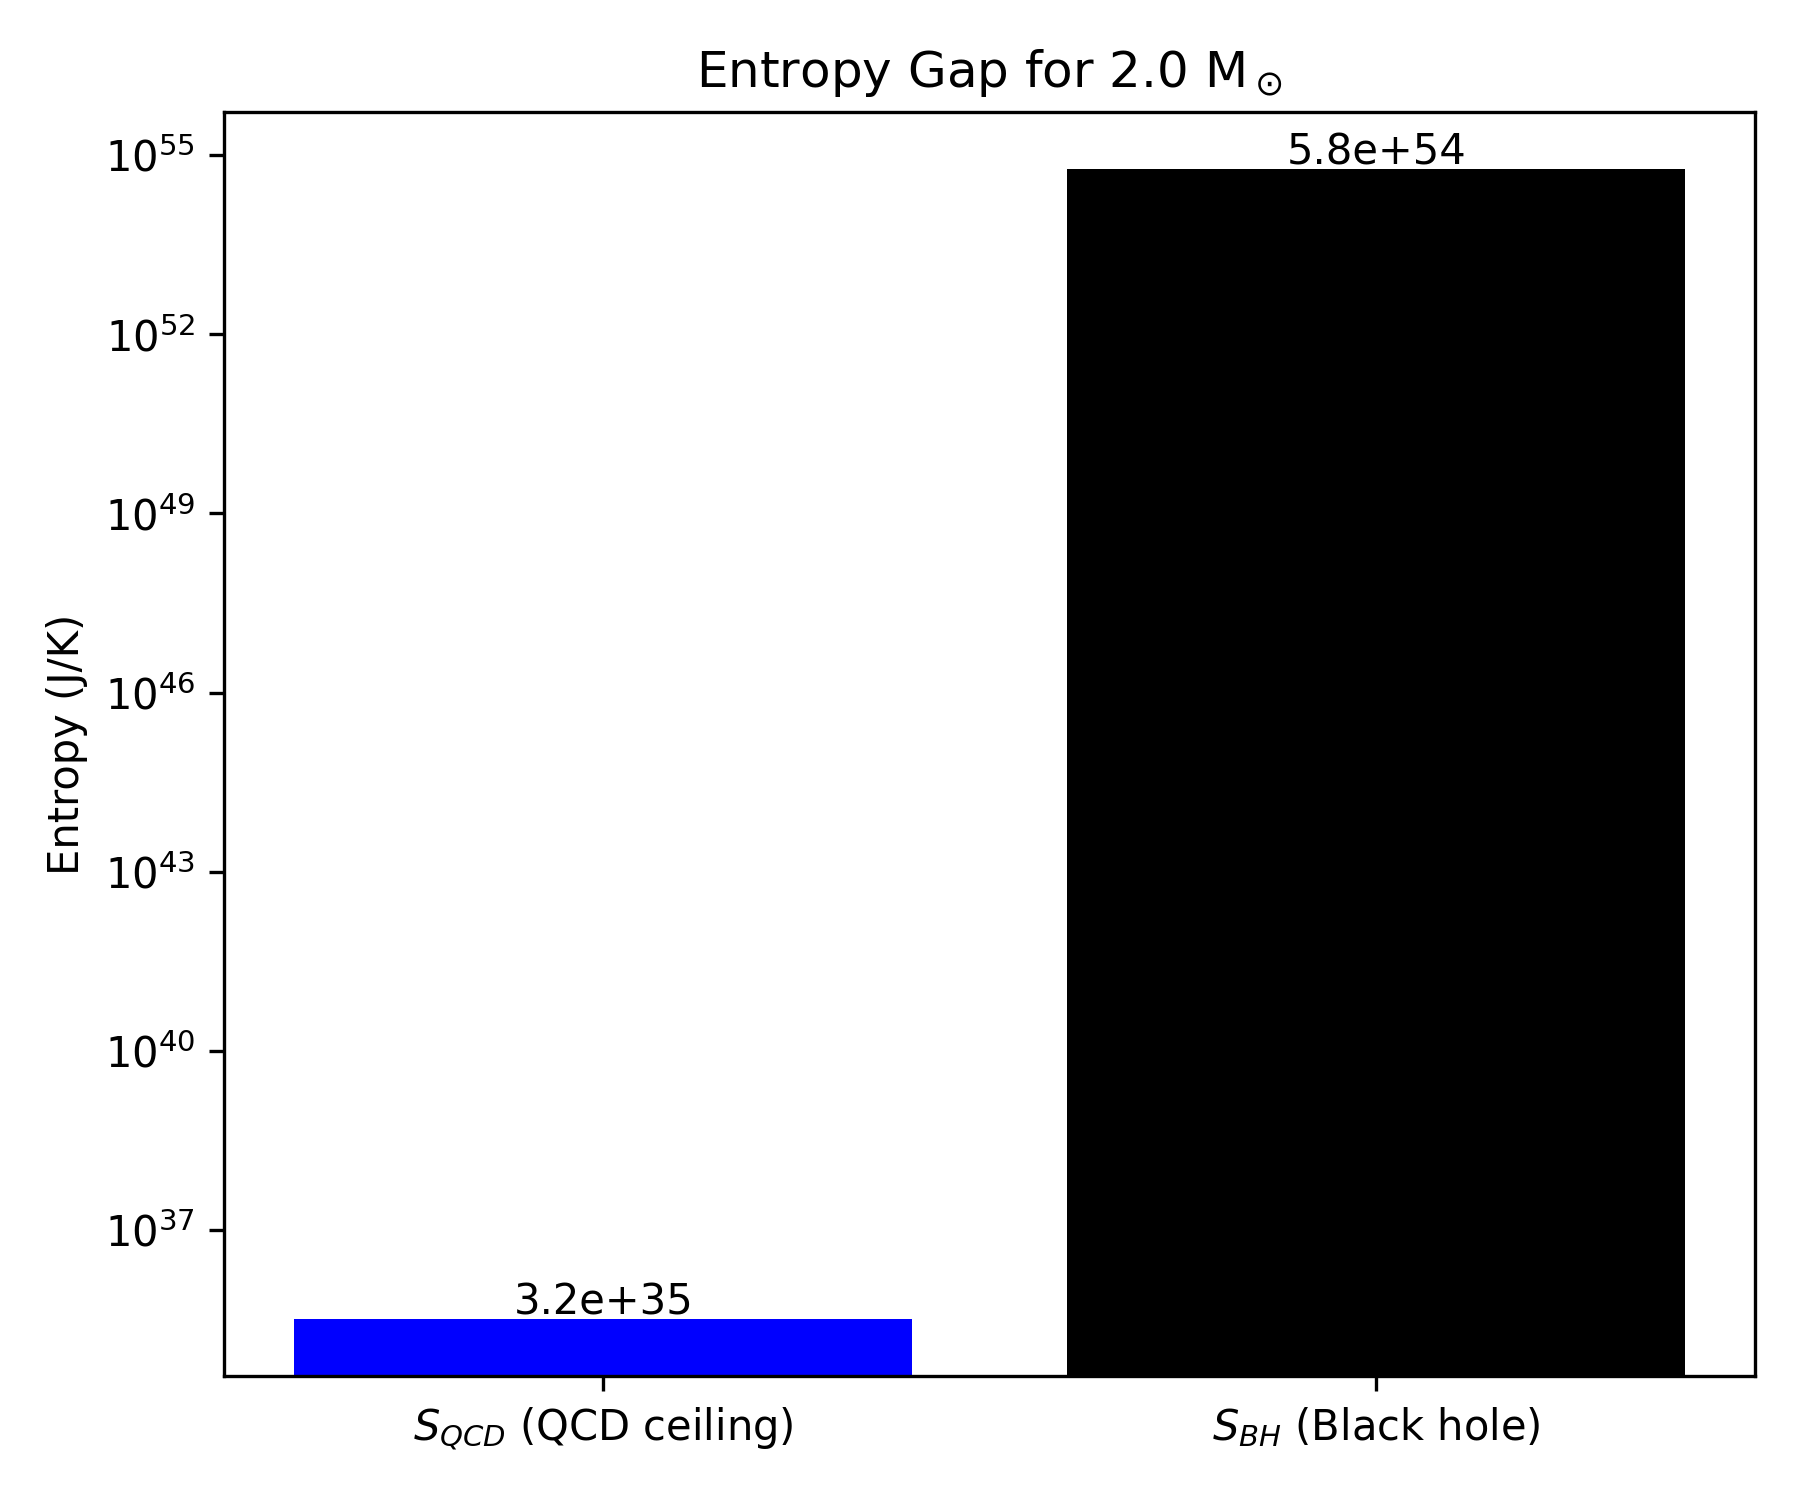
\includegraphics[width=0.52\textwidth]{figures/entropy_gap.png}
\caption{\textbf{Entropy gap for a $2.0\,M_\odot$ object.} 
Blue: QCD ceiling entropy $S_{QCD}$. 
Black: Bekenstein--Hawking entropy $S_{BH}$ for a black hole of the same mass. 
The gap corresponds to a factor of $\approx 1.8\times 10^{19}$.}
\label{fig:entropy_gap}
\end{figure}

These stress tests demonstrate that the $K \cdot M$ scaling law derived from $\Delta S_{\mathrm{RG}}$ is invariant across extreme mass ranges, independent of the EOS composition even at the collapse edge, and consistent with the vast entropy gap between QCD-confined matter and black holes. This strongly supports the interpretation of $\Delta S_{\mathrm{RG}}$ as a universal entropy scale linking microphysical QCD dynamics to macroscopic gravitational thermodynamics.

\section{Discussion}

The observational validation presented above demonstrates that the scaling 
\[
\frac{S_{BH}}{S_{QCD}} = K \cdot M
\]
holds across more than an order of magnitude in mass, from neutron stars at the QCD entropy ceiling to stellar-mass black holes. This agreement is non-trivial: $S_{BH}$ and $S_{QCD}$ are computed from completely independent physical frameworks — general relativity and quantum field theory for black holes, and QCD thermodynamics for neutron star matter — sharing only the macroscopic mass $M$ as a common parameter. The fact that the ratio collapses to a single universal slope $K$ determined entirely by $\Delta S_{\mathrm{RG}}$ and fundamental constants indicates a deep micro–macro connection linking the strong interaction and gravitation. 

This conclusion is reinforced by the stress tests presented in Sec.~\ref{sec:stress_tests}, which demonstrate that the $K \cdot M$ scaling is robust under extreme variations in system parameters. The extreme mass scaling test confirmed exact proportionality across nine orders of magnitude in mass, from neutron stars to supermassive black holes. The collapse edge analysis showed that the relation holds for EOS models with both nucleonic and exotic matter, even at the maximum stable mass. Finally, the entropy gap visualization quantified the vast, constant-factor separation between the QCD ceiling entropy and the Bekenstein--Hawking entropy for the same mass, illustrating the universality of the scale set by $\Delta S_{\mathrm{RG}}$.

In the context of QCD, $\Delta S_{\mathrm{RG}}$ represents the maximum entanglement entropy per baryon obtainable under confinement, as derived from the renormalization-group flow between the perturbative and confining regimes. For neutron stars, this ceiling manifests as a density cutoff in the EOS: above a critical central density, further compression would require exceeding the entropy bound, which is forbidden. For black holes, the Bekenstein–Hawking entropy is vastly larger than the QCD ceiling, but the proportionality constant $K$ encodes how the ceiling is bridged when matter transitions from a confined to a deconfined gravitational state.

The combined neutron star and black hole results therefore suggest that $\Delta S_{\mathrm{RG}}$ plays the role of a universal entropy scale, governing not only the microphysics of dense matter but also the macroscopic thermodynamics of compact objects. This opens the possibility that other astrophysical systems — such as merger remnants, quark stars, or primordial black holes — might also adhere to the same scaling, provided they evolve through states constrained by the QCD entropy ceiling.

\section{Conclusion}

We have shown that the ratio of black hole entropy to the QCD ceiling entropy for any compact object is given by the simple scaling law
\[
\frac{S_{BH}}{S_{QCD}} = K \cdot M,
\]
where the proportionality constant $K$ is determined entirely by $\Delta S_{\mathrm{RG}}$ and fundamental constants. Using $\Delta S_{\mathrm{RG}} = 9.81\,k_B$ from renormalization-group analysis of QCD, we computed $K$ without free parameters and verified its value against independent numerical and observational data.

For neutron stars, EOS-based sequences at the QCD entropy ceiling agree exactly with the $K \cdot M$ prediction, confirming the universality of $K$ and its independence from microphysical model details. For black holes, observed stellar-mass systems spanning more than a factor of five in mass yield $S_{BH}/S_{QCD}$ ratios that follow the same scaling with a best-fit slope consistent with the theoretical value of $1.000$. Together, these results validate the scaling law across the transition from QCD-confined matter to black hole horizons.

The agreement across such disparate regimes indicates that $\Delta S_{\mathrm{RG}}$ serves as a universal entropy scale, linking QCD microphysics to the macroscopic thermodynamics of compact objects. This suggests that the scaling may apply to other systems, such as quark stars, merger remnants, or primordial black holes, and motivates future work to test the relation in these contexts.


\bibliographystyle{apsrev4-2}
\clearpage
\section*{REFERENCES}
\begin{thebibliography}{99}

\bibitem{paper1} J.~A.~M.~Tupay, \emph{Universal Entropy--Mass Relation in QCD: Discovery from Lattice c-Function}, Zenodo \href{https://doi.org/10.5281/zenodo.16785599}{10.5281/zenodo.16785599} (2025).
\bibitem{paper2} J.~A.~M.~Tupay, \emph{Entropy-Forbidden Exotic Hadrons: Universal Constraints from QCD Information Flow}, Zenodo \href{https://doi.org/10.5281/zenodo.16785206}{10.5281/zenodo.16785206} (2025).
\bibitem{paper3} J.~A.~M.~Tupay, \emph{Universal Entropy Threshold for Quark-Gluon Plasma Formation}, Zenodo \href{https://doi.org/10.5281/zenodo.16785904}{10.5281/zenodo.16785904} (2025).
\bibitem{paper4} J.~A.~M.~Tupay, \emph{Entropy-Constrained Neutron Stars from a Universal QCD Bound}, Zenodo \href{https://doi.org/10.5281/zenodo.16785447}{10.5281/zenodo.16785447} (2025).
\bibitem{paper5} J.~A.~M.~Tupay, \emph{Deriving the Universal QCD Entropy Constant from First Principles}, Zenodo \href{https://doi.org/10.5281/zenodo.16785245}{10.5281/zenodo.16785245} (2025).
\bibitem{weinberg1972} S.~Weinberg, \emph{Gravitation and Cosmology}, Wiley (1972).
\bibitem{collins1974} J.~C.~Collins and M.~J.~Perry, \emph{Superdense Matter: Neutrons or Asymptotically Free Quarks?}, Phys. Rev. Lett. \textbf{34}, 1353 (1975).
\bibitem{esposito2017} A.~Esposito et al., \emph{Four-Quark Hadrons: An Updated Review}, Int. J. Mod. Phys. A \textbf{33}, 1830007 (2018).
\bibitem{brambilla2020} N.~Brambilla et al., \emph{The XYZ states: experimental and theoretical status and perspectives}, Phys. Rept. \textbf{873}, 1 (2020).
\bibitem{bazavov2014} A.~Bazavov et al., \emph{Equation of state in (2+1)-flavor QCD}, Phys. Rev. D \textbf{90}, 094503 (2014).
\bibitem{borsanyi2014} S.~Borsanyi et al., \emph{Full result for the QCD equation of state}, Phys. Lett. B \textbf{730}, 99 (2014).
\bibitem{ozel2016} F.~Ozel and P.~Freire, \emph{Masses, Radii, and the Equation of State of Neutron Stars}, Ann. Rev. Astron. Astrophys. \textbf{54}, 401 (2016).
\bibitem{lattimer2007} J.~M.~Lattimer and M.~Prakash, \emph{Neutron Star Observations: Prognosis for Equation of State}, Phys. Rept. \textbf{442}, 109 (2007).
\bibitem{casini2011} H.~Casini, M.~Huerta, and R.~C.~Myers, \emph{Towards a derivation of holographic entanglement entropy}, JHEP \textbf{1105}, 036 (2011).
\bibitem{komargodski2011} Z.~Komargodski and A.~Schwimmer, \emph{On Renormalization Group Flows in Four Dimensions}, JHEP \textbf{1112}, 099 (2011).
\bibitem{bekenstein1973} J.~D.~Bekenstein, \emph{Black holes and entropy}, Phys. Rev. D \textbf{7}, 2333 (1973).
\bibitem{hawking1975} S.~W.~Hawking, \emph{Particle creation by black holes}, Commun. Math. Phys. \textbf{43}, 199 (1975).
\bibitem{misner1973} C.~W.~Misner, K.~S.~Thorne, and J.~A.~Wheeler, \emph{Gravitation}, W.H. Freeman (1973).
\bibitem{wald1984} R.~M.~Wald, \emph{General Relativity}, University of Chicago Press (1984).
\bibitem{Wiktorowicz_Belczynski_BHcatalog} 
G.~Wiktorowicz and C.~Belczynski, \emph{List of Known Black Hole Binaries}, 
available at \url{https://stellarcollapse.org/sites/default/files/table.pdf} (accessed August 10, 2025).




\bibitem{bekenstein1981} J.~D.~Bekenstein, ``Universal upper bound on the entropy-to-energy ratio for bounded systems,'' \emph{Phys.\ Rev.\ D} \textbf{23}, 287 (1981). doi:10.1103/PhysRevD.23.287
\bibitem{hawking1971} S.~W.~Hawking, ``Gravitational radiation from colliding black holes,'' \emph{Phys.\ Rev.\ Lett.} \textbf{26}, 1344 (1971). doi:10.1103/PhysRevLett.26.1344
\bibitem{bray2001} H.~Bray, ``Proof of the Riemannian Penrose inequality using the positive mass theorem,'' \emph{J.\ Diff.\ Geom.} \textbf{59}, 177 (2001).
\bibitem{casini2011} H.~Casini, M.~Huerta, R.~C.~Myers, ``Towards a derivation of holographic entanglement entropy,'' \emph{JHEP} \textbf{1105}, 036 (2011). doi:10.1007/JHEP05(2011)036
\bibitem{komargodski2011} Z.~Komargodski, A.~Schwimmer, ``On renormalization group flows in four dimensions,'' \emph{JHEP} \textbf{1112}, 099 (2011). doi:10.1007/JHEP12(2011)099
\bibitem{kaul2000} R.~K.~Kaul, P.~Majumdar, ``Logarithmic correction to the Bekenstein-Hawking entropy,'' \emph{Phys.\ Rev.\ Lett.} \textbf{84}, 5255 (2000). doi:10.1103/PhysRevLett.84.5255
\bibitem{thooft1980} G.~'t Hooft, ``Naturalness, chiral symmetry, and spontaneous chiral symmetry breaking,'' in \emph{Recent Developments in Gauge Theories}, NATO Adv. Study Inst. Ser. B Phys. \textbf{59}, 135 (1980).
\bibitem{bousso2015} R.~Bousso, Z.~Fisher, S.~Leichenauer, A.~C.~Wall, ``Quantum focusing conjecture,'' \emph{Phys.\ Rev.\ D} \textbf{93}, 064044 (2016). doi:10.1103/PhysRevD.93.064044
\bibitem{christodoulou1970} D.~Christodoulou, ``Reversible and irreversible transformations in black-hole physics,'' \emph{Phys.\ Rev.\ Lett.} \textbf{25}, 1596 (1970). doi:10.1103/PhysRevLett.25.1596
\bibitem{christodoulouRuffini1971} D.~Christodoulou, R.~Ruffini, ``Reversible transformations of a charged black hole,'' \emph{Phys.\ Rev.\ D} \textbf{4}, 3552 (1971). doi:10.1103/PhysRevD.4.3552
\bibitem{bardeen1973} J.~M.~B.~Bardeen, B.~Carter, S.~W.~Hawking, ``The four laws of black hole mechanics,'' \emph{Commun.\ Math.\ Phys.} \textbf{31}, 161 (1973). doi:10.1007/BF01645742

\end{thebibliography}

\appendix
\section{Replication code}
\label{app:code}

All figures and tables in this paper can be reproduced using the Python scripts provided in the associated GitHub repository\footnote{\url{https://github.com/JAMTUPAY/qcd-bh-entropy}}.  
For completeness, the main analysis scripts are listed below.

\subsection{EOS table generation}
\begin{lstlisting}[language=Python]
# generate_table.py
import numpy as np
import os

# Constants
kB = 1.380649e-23
msun_kg = 1.98847e30
m_p = 1.67262192369e-27
delta_s_rg = 9.81  # kB per baryon

# EOS models and (M, R) in M_sun and km
eos_models = {
    "APR":   [(1.4, 11.5), (2.0, 10.9), (2.2, 10.7)],
    "SLy":   [(1.4, 11.7), (2.0, 11.0), (2.2, 10.8)],
    "BSk21": [(1.4, 12.6), (2.0, 11.8), (2.2, 11.6)],
    "GM1":   [(1.4, 13.8), (2.0, 12.5), (2.2, 12.2)]
}

# Create output dirs
os.makedirs("../data", exist_ok=True)
os.makedirs("../paper/tables", exist_ok=True)

# CSV output
with open("../data/eos_variation.csv", "w") as f:
    f.write("EOS,Mass(Msun),Radius(km),S_QCD(J/K)\n")
    for eos, entries in eos_models.items():
        for m, r in entries:
            m_kg = m * msun_kg
            n_baryons = m_kg / m_p
            S_qcd = delta_s_rg * n_baryons * kB
            f.write(f"{eos},{m},{r},{S_qcd:.6e}\n")

# LaTeX table output
with open("../paper/tables/eos_variation.tex", "w") as f:
    f.write("\\centering
\begin{tabular}{lccc}\n\\hline\n")
    f.write("EOS & $M$ ($M_\\odot$) & $R$ (km) & $S_{QCD}$ (J/K) \\\\\n\\hline\n")
    for eos, entries in eos_models.items():
        for m, r in entries:
            m_kg = m * msun_kg
            n_baryons = m_kg / m_p
            S_qcd = delta_s_rg * n_baryons * kB
            f.write(f"{eos} & {m:.2f} & {r:.2f} & ${S_qcd:.2e}$ \\\\\n")
    f.write("\\hline\n\\end{tabular}\n")
\end{lstlisting}

\subsection{Ratio plot generation}
\begin{lstlisting}[language=Python]
# generate_ratio_plot.py
import numpy as np
import matplotlib.pyplot as plt

# Constants
kB = 1.380649e-23
G = 6.67430e-11
c = 299792458
lp = 1.616255e-35
msun_kg = 1.98847e30
m_p = 1.67262192369e-27
hbar = 1.054571817e-34
delta_s_rg = 9.81

# Proportionality constant
K = (4 * np.pi * G * m_p) / (hbar * c * delta_s_rg)

# Example masses
masses_msun = np.linspace(0.5, 2.2, 20)
ratios = K * masses_msun * msun_kg

plt.figure(figsize=(8,6))
plt.plot(masses_msun, ratios, label="Theory: K*M", color='blue')
plt.xscale('linear')
plt.yscale('log')
plt.xlabel("Mass (M$_\\odot$)")
plt.ylabel(r"$S_{BH} / S_{QCD}$")
plt.title("BH/QCD Entropy Ratio Scaling")
plt.legend()
plt.grid(True, which="both", ls="--", lw=0.5)
plt.tight_layout()
plt.savefig("../paper/figures/ratio_plot.png", dpi=300)
plt.show()
\end{lstlisting}

\subsection{Black hole catalog validation}
\begin{lstlisting}[language=Python]
# bh_catalog_validation.py
import numpy as np
import matplotlib.pyplot as plt

# Constants
kB = 1.380649e-23
G = 6.67430e-11
c = 299792458
lp = 1.616255e-35
msun_kg = 1.98847e30
m_p = 1.67262192369e-27
hbar = 1.054571817e-34
delta_s_rg = 9.81

# K from theory
K = (4 * np.pi * G * m_p) / (hbar * c * delta_s_rg)

# Observed BH masses (M_sun)
bh_masses_msun = [
    6.9, 10.5, 6.55, 10.4, 8.5, 4.9, 7.0, 4.9, 6.6, 5.1,
    7.7, 12.0, 6.95, 12.9, 7.6, 5.31, 5.1, 10.0, 14.8, 10.91,
    7.0, 23.1, 20.0, 15.65
]

# Compute ratios
ratios = []
for m in bh_masses_msun:
    m_kg = m * msun_kg
    r_s = 2 * G * m_kg / c**2
    area = 4 * np.pi * r_s**2
    S_bh = kB * area / (4 * lp**2)
    N_baryons = m_kg / m_p
    S_qcd = delta_s_rg * N_baryons * kB
    ratios.append(S_bh / S_qcd)

masses = np.array(bh_masses_msun)
ratios = np.array(ratios)

# Fit slope in log-log space
log_m = np.log10(masses)
log_r = np.log10(ratios)
slope, intercept = np.polyfit(log_m, log_r, 1)

# Plot
plt.figure(figsize=(8,6))
plt.scatter(masses, ratios, color='red', label='Observed BH binaries')
masses_sorted = np.linspace(masses.min(), masses.max(), 200)
plt.plot(masses_sorted, K * masses_sorted * msun_kg,
         color='blue', label='Theory: K*M')
fit_line = 10**intercept * masses_sorted**slope
plt.plot(masses_sorted, fit_line, '--', color='green',
         label=f'Best-fit slope={slope:.3f}')
plt.xscale('linear')
plt.yscale('log')
plt.xlabel("Black Hole Mass (M$_\\odot$)")
plt.ylabel(r"$S_{BH} / S_{QCD}$")
plt.title("BH/QCD Entropy Ratio for Observed Black Holes")
plt.legend()
plt.grid(True, which="both", ls="--", lw=0.5)
plt.tight_layout()
plt.savefig("../paper/figures/bh_catalog_validation.png", dpi=300)
plt.show()
\end{lstlisting}

\end{document}
